% !TEX TS-program = Xelatex
% !TEX encoding = UTF-8 Unicode

\documentclass[UTF8]{ctexart}
\usepackage{amsmath}
\usepackage[bottom]{footmisc}
\usepackage{geometry}
\usepackage{graphicx}
\usepackage{figsize}
\usepackage[separate-uncertainty = true,per-mode=symbol]{siunitx}
\usepackage{tabu}
\usepackage{wasysym}
\geometry{left=0.7in,right=0.7in,bottom=0.7in,top=0.7in}

\title{实验十七:RLC串联电路的谐振}
\author{朱寅杰 1600017721}
\date{2017年12月1日}

\begin{document}
\maketitle
将一个电阻$R$、一个电感$L$、一个电容$C$串联接在一个交流信号源两端。调节信号源的频率直至电路达到谐振状态。记录此时信号发生器的频率,并用数字万用表分别测出电容$C$、电阻$R$与整个串联电路两端的电压的有效值$U_C$、$U_R$、$U$。我们需要计算这个共振系统的品质因子$Q$。单凭电路谐振时的状态,有两种计算方法:一种是由品质因子$Q$等于系统总储能与每$\frac{1}{2\pi}$周期内的耗能的比值得到$Q=\frac{LI^2}{I^2R/\omega_0}=\frac{L\omega_0}{R}=\frac{1}{R\omega_0C}$。

另一种算法是利用在达到谐振时,$L$与$C$上的电压均被放大为路端电压$U$的$Q$倍(这一性质可用于放大交流信号),于是有$Q=U_L/U=U_C/U$。由于实验使用的电感绕线的电阻较大(标称\SI{20}{\ohm},实际用万用表粗测为\SI{19.4}{\ohm}),因此其阻抗有一个较大的实部,相比之下,电容的阻抗可认为完全是由理想电容所贡献的,因此选用$U_C/U$作为$Q$的计算值。

判断达到谐振状态的依据是电路两端电压与电路中的电流同相位,在示波器上表现为李萨如图形退化为直线。由于测量时示波器屏幕上显示的信号噪声较大,无法获得明晰而锐利的图形,因此导致在信号源频率在\SI{2260}{\Hz}到\SI{2261}{\Hz}之间时示波器上显示的都是一条带有噪声的直线,单凭李萨如图形已经难以再对谐振频率有更精确的估计了,因此只好取$f_0=\SI{2260.5}{\Hz}$,其不确定度按从\SI{2260}{\Hz}到\SI{2261}{\Hz}的均匀分布计,为\SI{.3}{\Hz}。故$f_0=\SI{2260.5(3)}{\Hz}$。

所使用的电阻标称为\SI{100}{\ohm},有\SI{.01}{\ohm}的允差,故取$r=\SI{100.000(6)}{\ohm}$。注意由于电感和电容的阻抗也有实部,这个$r$并不是$Q$值计算式中的电路总电阻$R$。电路总电阻应由$R=r\frac{U}{U_R}$间接算出。所使用的电感标称\SI{.1}{H},有0.1\%的允差,故取$L=\SI{.10000(6)}{H}$。电容由电容箱提供一个\SI{.05}{\micro\F}的电容,其允差为0.65\%,故取$C=\SI{.0500(2)}{\micro\F}$。所使用的数字万用表为0.2\%+10个字。在谐振时测得标称电阻两端的电压$U_r=\SI{444.80}{\mV}$,$U_C=\SI{6.2448}{\V}$,$U=\SI{597.78}{\mV}$。将仪器允差折算入不确定度,得到$U_r=\SI{444.8(6)}{\mV}$,$U_C=\SI{6.245(7)}{\V}$,$U=\SI{597.8(7)}{\mV}$。按第一种办法,分别从电容和电感出发计算Q值:
\[Q=\frac{L\omega_0}{R}=\frac{2\pi fL}{r}\frac{U_r}{U}=\num{10.57(2)}\]
\[Q=\frac{1}{R\omega_0C}=\frac{1}{2\pi frC}\frac{U_r}{U}=\num{10.48(4)}\]
按第二种方法,从电压放大倍数计算$Q$值:
\[Q=U_C/U=\num{10.45(2)}\]


\subsection{相频曲线的绘制}
使用示波器分别监测$U$与$U_r$的信号,并在屏幕上通过定位点功能测出两信号的相位差。由于实验使用的示波器的内置时钟似乎出了点问题,因此同时测量了信号的周期$T$和两路信号的时间差$\Delta$,则相位差$\phi=\ang{360}\times\Delta/T$(取正号表示$U$超前$U_r$)。表中的有效数字按示波器测量的精度保留。将所测得的点用样条函数内插,绘制出$\phi-f$曲线在附图(a)中。

\begin{tabu} to 0.8\linewidth {X[c]|X[c] X[c]|X[c]}
\hline
输入频率$f$/Hz	&信号周期$T/\si{\micro\second}$	&时间差$\Delta/\si{\micro\second}$	&相位差$\phi/\deg$\\
\hline
1752	&604	&-139.5	&-83.1\\
1982	&524	&-107.5	&-73.9\\
2082	&497	&-89.0	&-64.5\\
2166	&477	&-63.0	&-47.5\\
2196	&469	&-48.5	&-37.2\\
2226	&463	&-31.0	&-24.1\\
2240	&452	&-15.5	&-12.3\\
(2260.5)	&&	&0\\
2282	&445.0	&23.0	&18.6\\
2310	&439.0	&38.5	&31.6\\
2350	&430.5	&56.0	&46.8\\
2440	&417.0	&74.0	&63.9\\
2590	&393.5	&83.5	&76.4\\
2917	&350.5	&85.5	&87.8\\
\hline
\end{tabu}

\subsection{幅频曲线的绘制}
改变发生器输出信号的频率,同时调节发生器输出信号的幅值,通过数字万用表监测路端输出电压的有效值保持在$U=\SI{597.4}{\milli\V}$,记录下$U_r$的值。测量使用的是万用表的AC电压档,然而测了一半忽然发现电压变成负的了,令人大惊失色,重置了一下仪器把之前的数据重新测量了一遍,发现之前的数据都比正确值小了大约\SI{87}{\milli\V}。难道说这个万用表的交流档还有零点校准一说?下次去翻一翻仪器的说明书,或许能找到这个bug的来源。

\begin{tabu}to .9\linewidth {X[-10,c]|X[c]X[c]X[c]X[c]X[c]X[c]X[c]X[c]X[c]X[c,-1]}
\hline
频率$f$/Hz	&1752&1867&1982&2032&2082&2124&2166&2181&2196\\
\hline
$U_r$/mV	&80.302&106.44&150.47&180.53&221.96&269.47&330.87&355.40&380.19\\
\hline\hline
频率$f$/Hz	&2226&2240&2250&2260&2261&2270&2282&2296&2310&\\
\hline
$U_r$/mV	&423.53&437.10&442.76&444.80&444.68&442.67&435.42&421.61&403.21&\\
\hline\hline
频率$f$/Hz	&2330&2350&2395&2440&2515&2590&2853&2917&\\
\hline
$U_r$/mV	&373.21&342.42&280.44&233.06&179.45&145.33&87.432&79.975&\\
\hline
\end{tabu}

同样使用样条函数内插绘制出的$U_r-f$图线如附图(b)。在图中读出内插的样条函数与$U_{max}/\sqrt{2}$水平线的两交点,横坐标分别为\SI{2368.9}{\Hz}与\SI{2155.8}{\Hz},从而计算出$Q=\frac{f_0}{\Delta f}=\frac{2260.5}{2368.9-2155.8}=10.61$。
\subsection{思考题}
如果把串联入的\SI{100}{\ohm}电阻替换成\SI{500}{\ohm},谐振频率将不会发生变化。而电路的品质因子$Q$反比于电路的总电阻。当接入的电阻为\SI{100}{\ohm}时电路总电阻为$R=r\frac{U}{U_R}=\SI{134}{\ohm}$,替换后自然变成\SI{534}{\ohm},故品质因子$Q$将从原来的10.5左右变为约2.6,变成原来的四分之一。由于$Q=f_0/\Delta f$,故一个只有2.6的品质因子意味着谐振峰会被削平。具体来说,$U_max/\sqrt{2}$的频带宽度会有大约\SI{850}{\Hz}宽,而谐振时电容上的电压的振幅相对路端电压的放大率会变为只有原来的四分之一。反映到曲线上,相频曲线和幅频曲线都好像被水平拉长到原来的四倍。

书中所示的测量$Q$值的装置的原理很简单,就是利用了前面提到的串联$RLC$电路达到谐振时,$L$与$C$上的电压均被放大为路端电压$U$的$Q$倍的性质。具体测量的办法是调节信号源使得在输出电压$u$不变的时候电容两端电压$u_C$取极大,当$Q$很大(谐振峰很尖时)可近似认为此时电路达到谐振,从而可以计算出$Q=u_C/u=100$。再由$Q=\frac{L\omega_0}{R}$得出$R=1/(2\pi Qf_0C)=\SI{8.04}{\ohm}$,$L=1/(4\pi^2f_0C)=\SI{0.213}{\milli H}$。
\begin{figure}
\centering
\SetFigLayout{2}{1}
\subfigure[相位差-频率曲线。图中竖直粗线为谐振频率。]{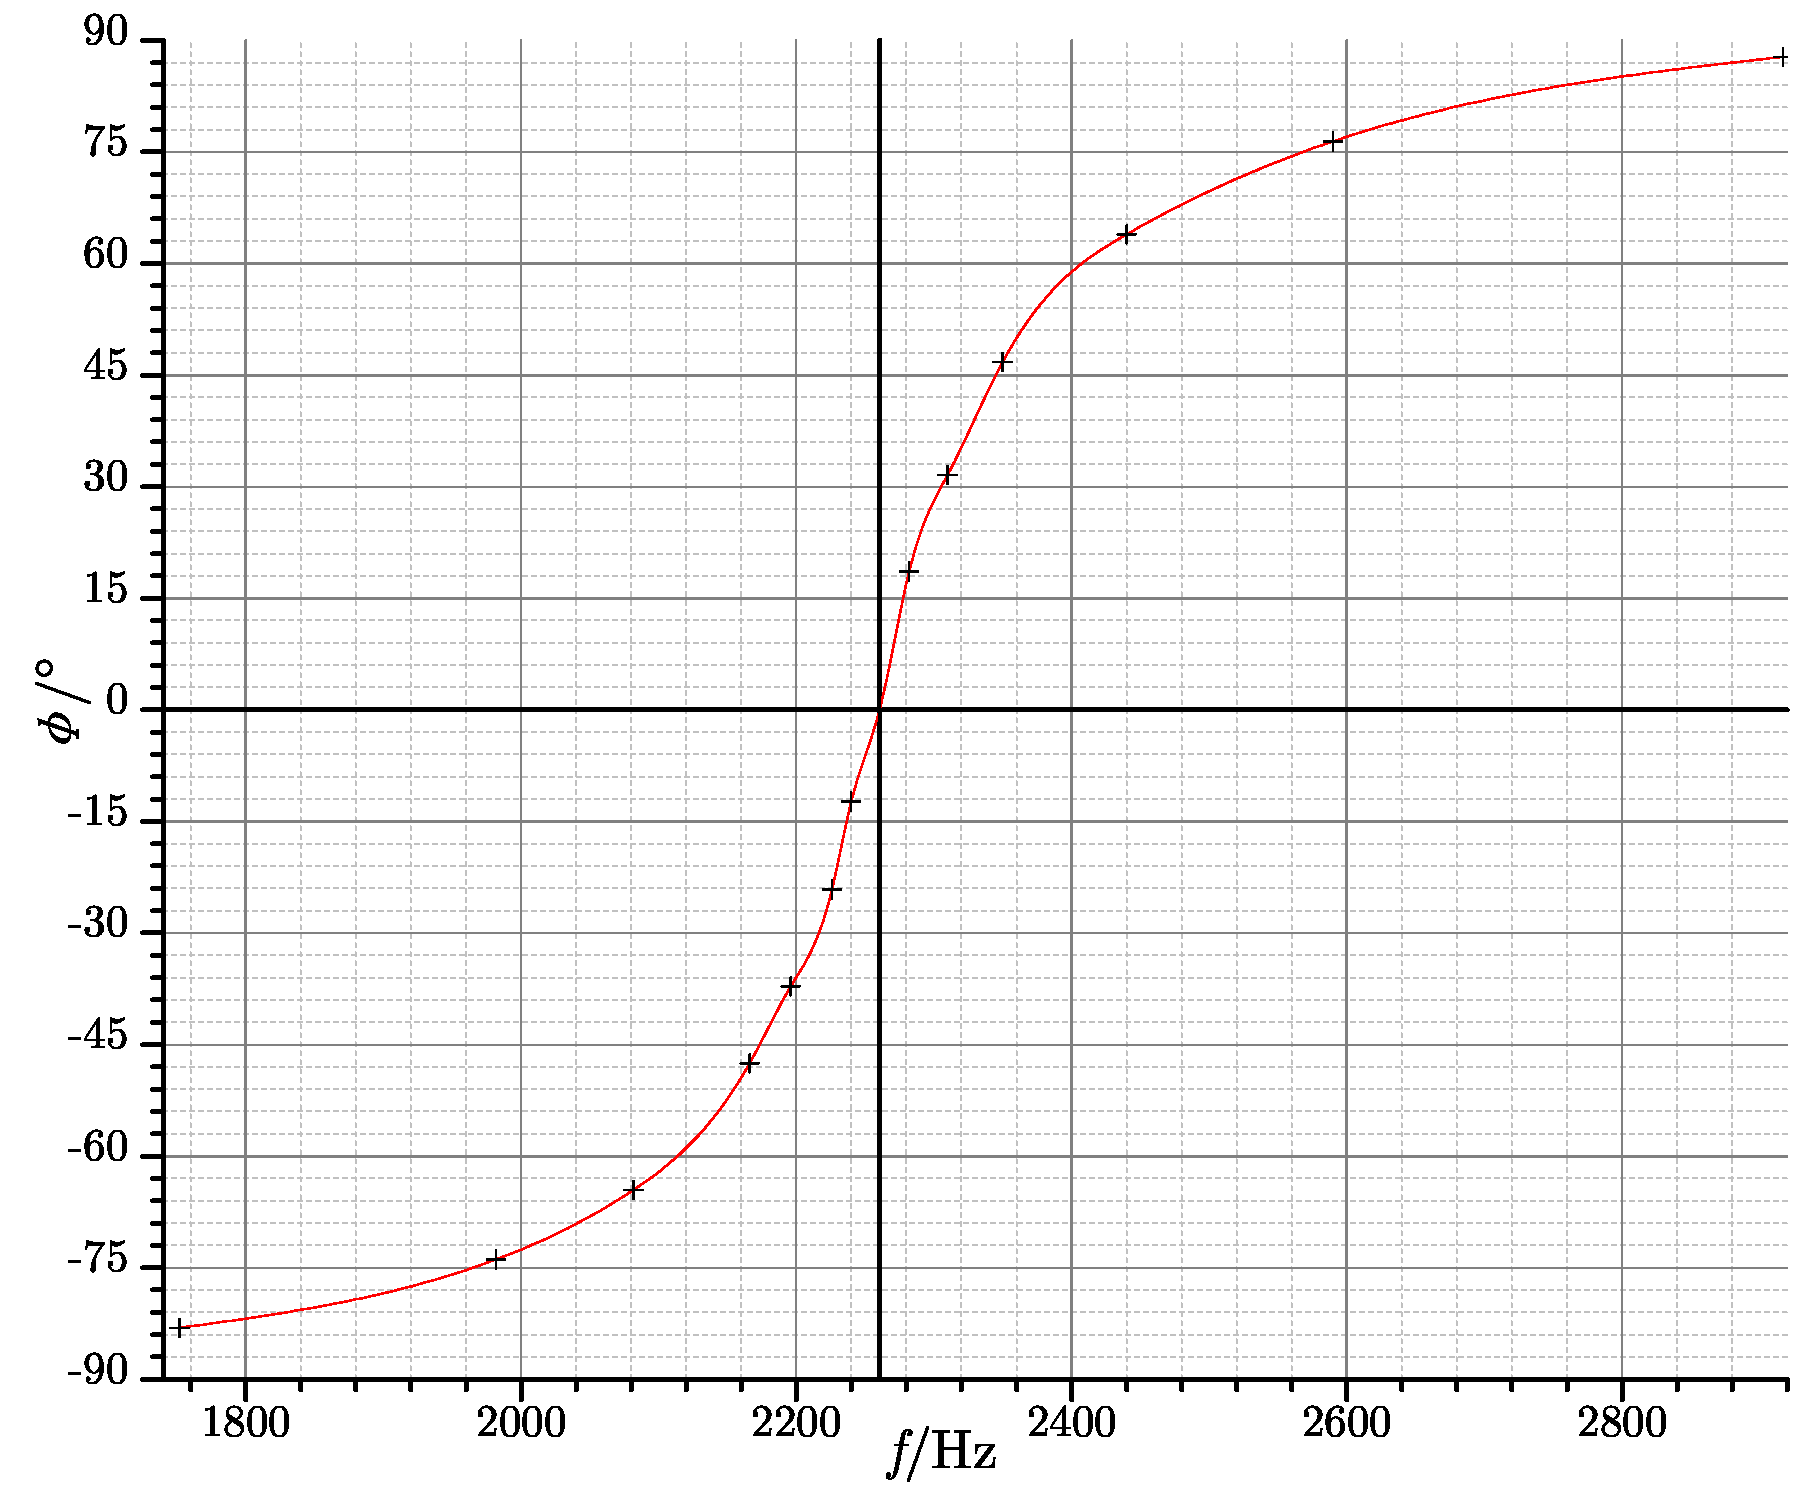
\includegraphics{phase.eps}} \\
\subfigure[电压幅度-频率曲线。纵轴为保持路端电压有效值$U=\SI{597.4}{\milli\V}$时测得的$U_r$的有效值。图中竖直粗线为谐振频率,水平粗线为谐振时电压的$1/\sqrt{2}$倍。]{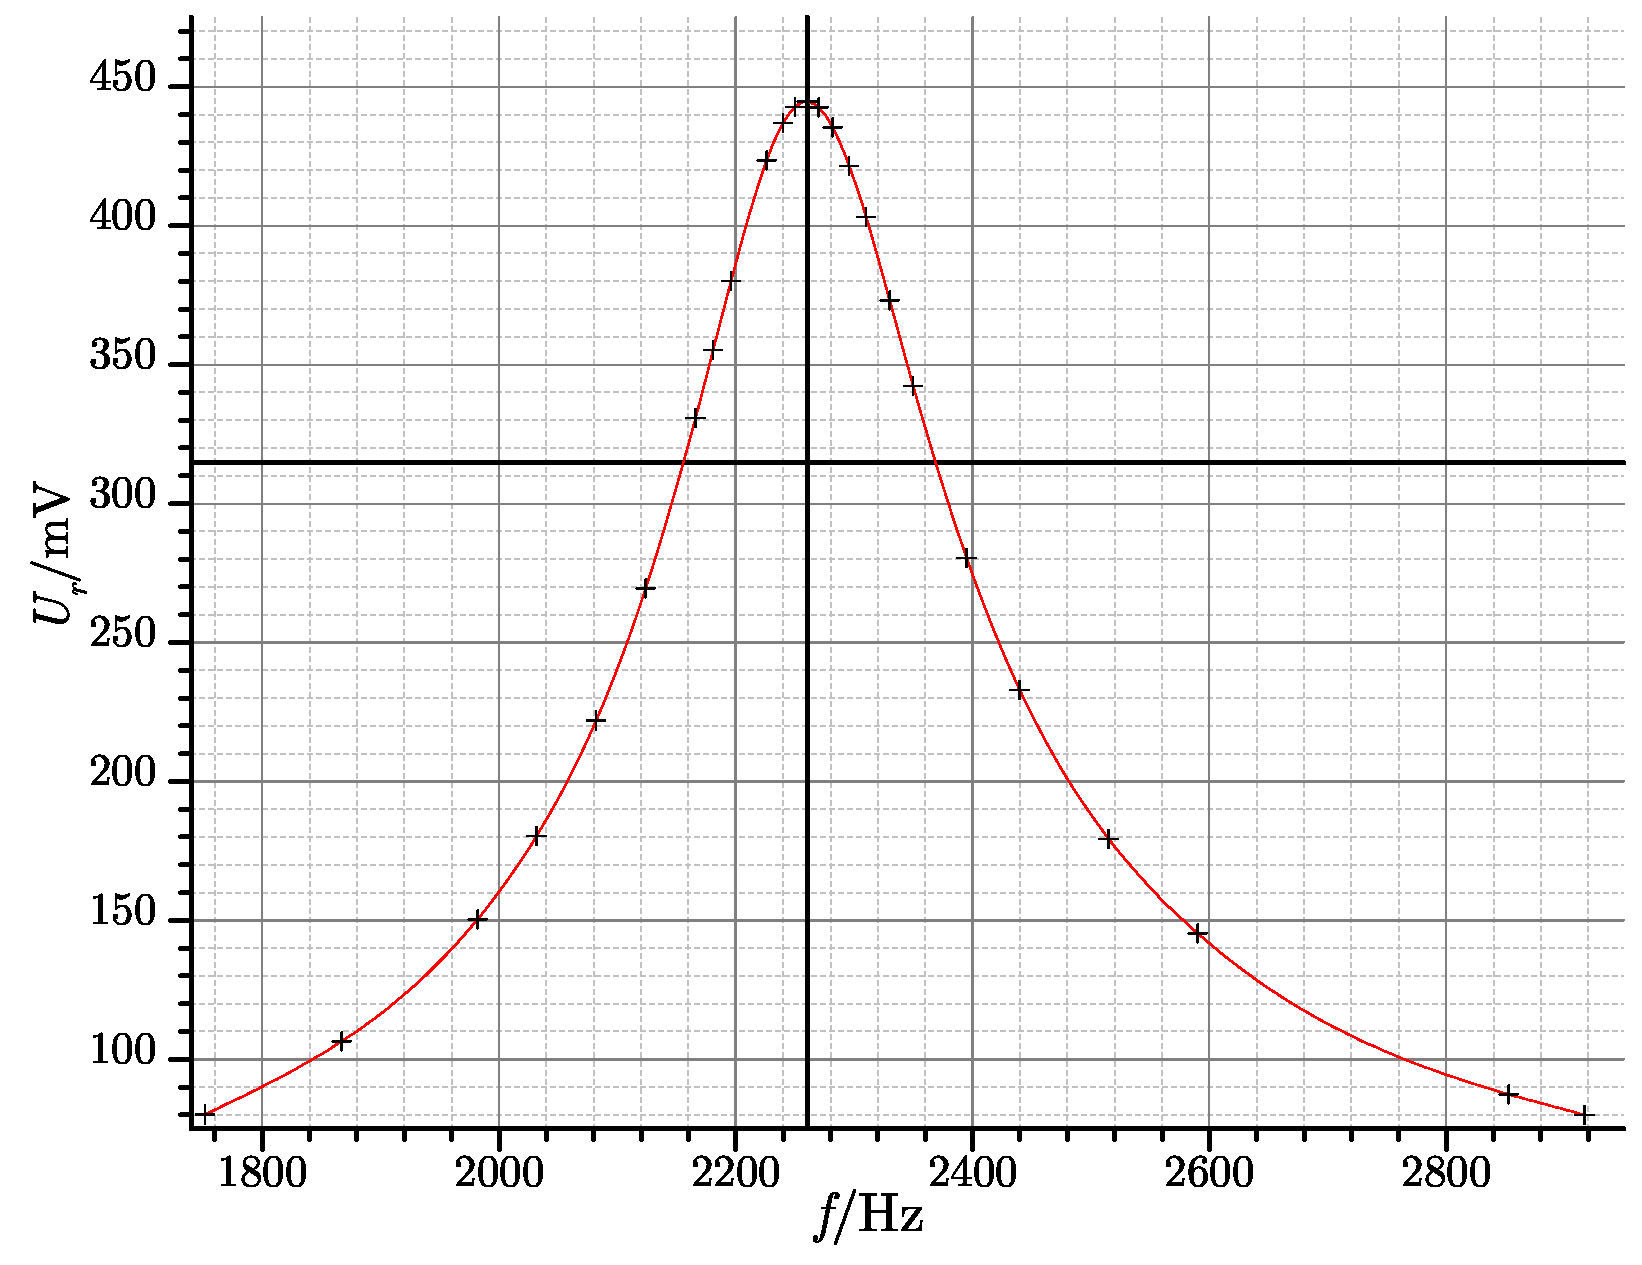
\includegraphics{amp.eps}} \\
\end{figure}
\end{document} 